%\clearpage
\section{Data processing details and antecedent mining}
\label{appendix:data}

\subsection{ProPublica recidivism dataset}
Table~\ref{tab:recidivism-data} shows the~6 attributes
and corresponding~17 categorical values
that we use for the ProPublica dataset.
%
From these, we construct~17 single-clause antecedents, \eg ${(age = 23-25)}$.
%
We then combine pairs of these antecedents as conjunctions to form
two-clause antecedents, \eg ${(age = 23-25) \wedge (priors = 2-3)}$.
%
By virtue of our lower bound on antecedent support,
(Theorem~\ref{thm:min-capture},~\S\ref{sec:lb-support}),
we eliminate antecedents with support less than~0.005 or greater than~0.995,
since ${\Reg = 0.005}$ is the smallest regularization parameter value
we study for this problem.
%
With this filtering step, we generate between~121 and~123 antecedents for each fold;
without it, we would instead generate about~130 antecedents as input to our algorithm.

Note that we exclude the `current charge' attribute (which has two categorical values,
`misdemeanor' and `felony'); for individuals in the dataset booked on multiple charges,
this attribute does not appear to consistently reflect the most serious charge.

\begin{table}[h!]
\centering
%$Q_\text{max}$ $K_\text{max}$
\begin{tabular}{l  | c  c  c}
Feature & Value range & Categorical values & Count \\
\hline
sex & --- & male, female & 2 \\
age & 18-96 & 18-20, 21-22, 23-25, 26-45, $>$45  & 5 \\
juvenile felonies & 0-20 & 0, $>$0 & 2 \\
juvenile misdemeanors & 0-13 & 0, $>$0 & 2 \\
%other juvenile crimes & 0-17 & --- & 2 \\
juvenile crimes & 0-21 & 0, $>$0 & 2 \\
priors & 0-38 & 0, 1, 2-3, $>$3 & 4
\end{tabular}
%\vspace{4mm}
\caption{Categorical features (6 attributes, 17 values) from the ProPublica dataset.
We construct the feature \emph{juvenile crimes} from the sum of
\emph{juvenile felonies}, \emph{juvenile misdemeanors}, and
the number of juvenile crimes that were neither felonies nor misdemeanors (not shown).
}
\vspace{4mm}
\label{tab:recidivism-data}
\end{table}

\subsection{NYPD stop-and-frisk dataset}
This dataset is larger than, but similar to the NYCLU stop-and-frisk dataset, 
described next.

%\newpage
\subsection{NYCLU stop-and-frisk dataset}
The original dataset contains 45,787 records,
each describing an incident involving a stopped person; the individual
was frisked in 30,345 (66.3\%) of records and and searched in 7,283 (15.9\%).
%
In 30,961 records, the individual was frisked and/or searched (67.6\%); of those,
a criminal possession of a weapon was identified 1,445 times (4.7\% of these records).
%
We remove 1,929 records with missing data, as well as a small number with extreme values
for the individual's age -- we eliminate those with age~${< 12}$ or~${>89}$.
%we also assume that one age marked `366' is a typo, and we replace it with `36'.
%
This yields a set of 29,595 records in which the individual was frisked and/or searched.
%
To address the class imbalance for this problem, we sample records from the
smaller class with replacement.
%
We generate cross-validation folds first, and then resample within each fold.
%
In our 10-fold cross-validation experiments, each training set contains 50,743 observations.
%
Table~\ref{tab:frisk-data} shows the 5 categorical attributes that we use,
corresponding to a total of 28 values.
%
Our experiments use these antecedents,
as well as negations of the 18 antecedents corresponding to the two features
\emph{stop reason} and \emph{additional circumstances},
which gives a total of 46 antecedents.

\begin{table}[h!]
\centering
%$Q_\text{max}$ $K_\text{max}$
\begin{tabular}{l | c  c}
Feature & Values & Count \\
\hline
stop reason & suspicious object, fits description, casing, & 9 \\
& acting as lookout, suspicious clothing, & \\
& drug transaction, furtive movements, & \\
& actions of violent crime, suspicious bulge \\
\hline
additional & proximity to crime scene, evasive response,  & 9 \\
circumstances & associating with criminals, changed direction, & \\
& high crime area, time of day,  & \\
& sights and sounds of criminal activity, & \\
& witness report, ongoing investigation & \\
\hline
city & Queens,  Manhattan, Brooklyn, Staten Island, Bronx & 5 \\
\hline
location & housing authority, transit authority, & 3 \\
& neither housing nor transit authority & \\
\hline
inside or outside & inside, outside & 2 \\
\end{tabular}
%\vspace{4mm}
\caption{Categorical features (5 attributes, 28 values) from the NYCLU dataset.}
\vspace{4mm}
\label{tab:frisk-data}
\end{table}

%\clearpage
\section{Example optimal rule lists, for different values of~$\Reg$}
\label{appendix:examples}

For each of our prediction problems, we provide listings of
optimal rule lists found by CORELS, across 10 cross-validation folds,
for different values of the regularization parameter~$\Reg$.
%
These rule lists correspond to the results for CORELS summarized
in Figures~\ref{fig:sparsity-compas} and~\ref{fig:sparsity-weapon}~(\S\ref{sec:sparsity}).
%
Recall that as~$\Reg$ decreases, optimal rule lists tend to grow in length. \\

\subsection{ProPublica recidivism dataset}
We show example optimal rule lists that predict two-year recidivism.
%
Figure~\ref{fig:recidivism-rule-list-02-01} shows examples for
regularization parameters~${\Reg = 0.02}$ and~0.01.
%
Figure~\ref{fig:recidivism-rule-list-005} shows examples for~${\Reg = 0.005}$;
Figure~\ref{fig:recidivism-all-folds}~(\S\ref{sec:examples}) showed two representative examples.

For the largest regularization parameter~${\Reg = 0.02}$~(Figure~\ref{fig:recidivism-rule-list-02-01}),
we observe that all folds identify the same length-1 rule list.
%
For the intermediate value~${\Reg = 0.01}$ (Figure~\ref{fig:recidivism-rule-list-02-01}),
the folds identify optimal 2-rule or 3-rule lists that contain the nearly same prefix rules,
up to permutations.
%
For the smallest value~${\Reg = 0.005}$~(Figure~\ref{fig:recidivism-rule-list-005}),
the folds identify optimal 3-rule or 4-rule lists that contain the nearly same prefix rules,
up to permutations.
%
Across all three regularization parameter values and all folds,
the prefix rules always predict the positive class label,
and the default rule always predicts the negative class label.
%
We note that our objective is not designed to enforce any of these properties.
%though some may be seen as desirable.

% tail -n 1 ../logs/for-compas_*_train.out-curious_lb-with_prefix_perm_map-minor-removed=none-max_num_nodes=10000000-c=0.0200000-v=progress-f=1000-opt.txt
%{priors:>3}~1;default~0
%
%$ tail -n 1 ../logs/for-compas_*_train.out-curious_lb-with_prefix_perm_map-minor-removed=none-max_num_nodes=10000000-c=0.0100000-v=progress-f=1000-opt.txt
%{priors:>3}~1;{sex:Male,juvenile-crimes:>0}~1;default~0 x 3
%{sex:Male,juvenile-crimes:>0}~1;{priors:>3}~1;default~0 x 2
%{sex:Male,age:18-20}~1;{priors:>3}~1;default~0 x 2
%{age:21-22,priors:2-3}~1;{priors:>3}~1;{sex:Male,age:18-20}~1;default~0 x 2
%{priors:>3}~1;{sex:Male,age:18-20}~1;default~0
\begin{figure}[h!]
\textbf{Two-year recidivism prediction $(\Reg = 0.02)$}
\vspace{1mm}
\begin{algorithmic}
\State \bif $(priors > 3)$ \bthen $yes$ \Comment{Found by all 10 folds}
\State \belse $no$
\end{algorithmic}
\vspace{5mm}
\textbf{Two-year recidivism prediction $(\Reg = 0.01)$}
\vspace{1mm}
\begin{algorithmic}
\State \bif $(priors > 3)$ \bthen $yes$ \Comment{Found by 3 folds}
\State \belif $(sex = male) \band (juvenile~crimes > 0)$ \bthen $yes$
\State \belse $no$
\end{algorithmic}
\vspace{1mm}
\begin{algorithmic}
\State \bif $(sex = male) \band (juvenile~crimes > 0)$ \bthen $yes$ \Comment{Found by 2 folds}
\State \belif $(priors > 3)$ \bthen $yes$
\State \belse $no$
\end{algorithmic}
\vspace{1mm}
\begin{algorithmic}
\State \bif $(age = 21-22) \band (priors = 2-3)$ \bthen $yes$ \Comment{Found by 2 folds}
\State \belif $(priors > 3)$ \bthen $yes$
\State \belif $(age = 18-20) \band (sex = male)$ \bthen $yes$
\State \belse $no$
\end{algorithmic}
\vspace{1mm}
\begin{algorithmic}
\State \bif $(age = 18-20) \band (sex = male)$ \bthen $yes$ \Comment{Found by 2 folds}
\State \belif $(priors > 3)$ \bthen $yes$
\State \belse $no$
\end{algorithmic}
\vspace{1mm}
\begin{algorithmic}
\State \bif $(priors > 3)$ \bthen $yes$ \Comment{Found by 1 fold}
\State \belif $(age = 18-20) \band (sex = male)$ \bthen $yes$
\State \belse $no$
\end{algorithmic}
\caption{Example optimal rule lists for the ProPublica dataset,
found by CORELS with regularization parameters~${\Reg = 0.02}$~(top),
and~0.01~(bottom) across 10 cross-validation folds.
}
\label{fig:recidivism-rule-list-02-01}
\end{figure}

%logs in jmlr/ from Nicholas 9/27
%$ tail -n 1 *compas*curious*with*-minor*none-m*1000000000*0.005*opt.txt
%{sex:Male,age:18-20}~1;{age:21-22,priors:2-3}~1;{priors:>3}~1;default~0 x 4
%{age:21-22,priors:2-3}~1;{priors:>3}~1;{sex:Male,age:18-20}~1;default~0 x 2
%{sex:Male,age:18-20}~1;{priors:>3}~1;{age:21-22,priors:2-3}~1;default~0
%{sex:Male,age:18-20}~1;{age:21-22,priors:2-3}~1;{age:23-25,priors:2-3}~1;{priors:>3}~1;default~0
%{sex:Male,age:18-20}~1;{age:21-22,priors:2-3}~1;{priors:>3}~1;{age:23-25,priors:2-3}~1;default~0
%{age:21-22,priors:2-3}~1;{age:23-25,priors:2-3}~1;{priors:>3}~1;{sex:Male,age:18-20}~1;default~0
\begin{figure}[h!]
\textbf{Two-year recidivism prediction $(\Reg = 0.005)$}
\vspace{1mm}
\begin{algorithmic}
\State \bif $(age = 18-20) \band (sex = male)$ \bthen $yes$ \Comment{Found by 4 folds}
\State \belif $(age = 21-22) \band (priors = 2-3)$ \bthen $yes$
\State \belif $(priors > 3)$ \bthen $yes$
\State \belse $no$
\end{algorithmic}
\vspace{1mm}
\begin{algorithmic}
\State \bif $(age = 21-22) \band (priors = 2-3)$ \bthen $yes$  \Comment{Found by 2 folds}
\State \belif $(priors > 3)$ \bthen $yes$
\State \belif $(age = 18-20) \band (sex = male)$ \bthen $yes$
\State \belse $no$
\end{algorithmic}
\vspace{1mm}
\begin{algorithmic}
\State \bif $(age = 18-20) \band (sex = male)$ \bthen $yes$ \Comment{Found by 1 fold}
\State \belif $(priors > 3)$ \bthen $yes$
\State \belif $(age = 21-22) \band (priors = 2-3)$ \bthen $yes$
\State \belse $no$
\end{algorithmic}
\vspace{1mm}
\begin{algorithmic}
\State \bif $(age = 18-20) \band (sex = male)$ \bthen $yes$ \Comment{Found by 1 fold}
\State \belif $(age = 21-22) \band (priors = 2-3)$ \bthen $yes$
\State \belif $(age = 23-25) \band (priors = 2-3)$ \bthen $yes$
\State \belif $(priors > 3)$ \bthen $yes$
\State \belse $no$
\end{algorithmic}
\vspace{1mm}
\begin{algorithmic}
\State \bif $(age = 18-20) \band (sex = male)$ \bthen $yes$ \Comment{Found by 1 fold}
\State \belif $(age = 21-22) \band (priors = 2-3)$ \bthen $yes$
\State \belif $(priors > 3)$ \bthen $yes$
\State \belif $(age = 23-25) \band (priors = 2-3)$ \bthen $yes$
\State \belse $no$
\end{algorithmic}
\vspace{1mm}
\begin{algorithmic}
\State \bif $(age = 21-22) \band (priors = 2-3)$ \bthen $yes$ \Comment{Found by 1 fold}
\State \belif $(age = 23-25) \band (priors = 2-3)$ \bthen $yes$
\State \belif $(priors > 3)$ \bthen $yes$
\State \belif $(age = 18-20) \band (sex = male)$ \bthen $yes$
\State \belse $no$
\end{algorithmic}
\caption{Example optimal rule lists for the ProPublica dataset,
found by CORELS with regularization parameters~${\Reg = 0.005}$,
across 10 cross-validation folds.
}
\label{fig:recidivism-rule-list-005}
\end{figure}

\clearpage
\subsection{NYPD stop-and-frisk dataset}
We show example optimal rule lists that predict whether a weapon
will be found on a stopped individual who is frisked or searched, learned from the NYPD dataset.

\begin{figure}[b!]
%$ head *cpw_*0.01*opt* K = 2
%{cs_objcs:stop-reason=suspicious-object}~1;{location:transit-authority}~1;default~0 x 8
%{location:transit-authority}~1;{cs_objcs:stop-reason=suspicious-object}~1;default~0 x 2
\textbf{Weapon prediction $(\Reg = 0.01, \text{Feature Set~C})$}
\vspace{1mm}
\begin{algorithmic}
\State \bif $(stop~reason = suspicious~object)$ \bthen $yes$ \Comment{Found by 8 folds}
\State \belif $(location = transit~authority)$ \bthen $yes$
\State \belse $no$
\end{algorithmic}
\vspace{1mm}
\begin{algorithmic}
\State \bif $(location = transit~authority)$ \bthen $yes$ \Comment{Found by 2 folds}
\State \belif $(stop~reason = suspicious~object)$ \bthen $yes$
\State \belse $no$
\end{algorithmic}
\vspace{5mm}
%$ head *cpw_*0.005*opt* K = 4 or 5
%{cs_objcs:stop-reason=suspicious-object}~1;{location:transit-authority}~1;{location:housing-authority}~0;{city:MANHATTAN}~1;default~0 x 7
%{cs_objcs:stop-reason=suspicious-object}~1;{location:housing-authority}~0;{location:transit-authority}~1;{city:MANHATTAN}~1;default~0
%{cs_objcs:stop-reason=suspicious-object}~1;{location:housing-authority}~0;{city:MANHATTAN}~1;{location:transit-authority}~1;default~0
%{cs_objcs:stop-reason=suspicious-object}~1;{location:transit-authority}~1;{city:BRONX}~0;{location:housing-authority}~0;{cs_furtv:stop-reason=furtive-movements}~0;default~1
\textbf{Weapon prediction $(\Reg = 0.005, \text{Feature Set~C})$}
\begin{algorithmic}
\State \bif $(stop~reason = suspicious~object)$ \bthen $yes$ \Comment{Found by 7 folds}
\State \belif $(location = transit~authority)$ \bthen $yes$
\State \belif $(location = housing~authority)$ \bthen $no$
\State \belif $(city = Manhattan)$ \bthen $yes$
\State \belse $no$
\end{algorithmic}
\vspace{1mm}
\begin{algorithmic}
\State \bif $(stop~reason = suspicious~object)$ \bthen $yes$ \Comment{Found by 1 fold}
\State \belif $(location = housing~authority)$ \bthen $no$
\State \belif $(location = transit~authority)$ \bthen $yes$
\State \belif $(city = Manhattan)$ \bthen $yes$
\State \belse $no$
\end{algorithmic}
\vspace{1mm}
\begin{algorithmic}
\State \bif $(stop~reason = suspicious~object)$ \bthen $yes$ \Comment{Found by 1 fold}
\State \belif $(location = housing~authority)$ \bthen $no$
\State \belif $(city = Manhattan)$ \bthen $yes$
\State \belif $(location = transit~authority)$ \bthen $yes$
\State \belse $no$
\end{algorithmic}
\vspace{1mm}
\begin{algorithmic}
\State \bif $(stop~reason = suspicious~object)$ \bthen $yes$ \Comment{Found by 1 fold}
\State \belif $(location = transit~authority)$ \bthen $yes$
\State \belif $(city = Bronx)$ \bthen $no$
\State \belif $(location = housing~authority)$ \bthen $no$
\State \belif $(stop~reason = furtive~movements)$ \bthen $no$
\State \belse $yes$
\end{algorithmic}
\caption{Example optimal rule lists for the NYPD stop-and-frisk dataset,
found by CORELS with regularization parameters~${\Reg = 0.01}$~(top) and~0.005~(bottom),
across 10 cross-validation folds.
}
\label{fig:cpw-rule-list}
\end{figure}

\begin{figure}[b!]
%$ head *cpw-noloc_*0.01*opt* K = 2
%{cs_objcs:stop-reason=suspicious-object}~1;{inout:outside}~0;default~1 x 7
%{cs_objcs:stop-reason=suspicious-object}~1;{inout:inside}~1;default~0 x 3
\textbf{Weapon prediction $(\Reg = 0.01, \text{Feature Set~D})$}
\vspace{1mm}
\begin{algorithmic}
\State \bif $(stop~reason = suspicious~object)$ \bthen $yes$ \Comment{Found by 7 folds}
\State \belif $(inside~or~outside = outside)$ \bthen $no$
\State \belse $yes$
\end{algorithmic}
\vspace{1mm}
\begin{algorithmic}
\State \bif $(stop~reason = suspicious~object)$ \bthen $yes$ \Comment{Found by 3 folds}
\State \belif $(inside~or~outside = inside)$ \bthen $yes$
\State \belse $no$
\end{algorithmic}
\vspace{5mm}
%$ head *cpw-noloc_*0.005*opt* K = 4
%{cs_objcs:stop-reason=suspicious-object}~1;{cs_lkout:stop-reason=acting-as-lookout}~0;{cs_descr:stop-reason=fits-description}~0;{cs_furtv:stop-reason=furtive-movements}~0;default~1 x 2
%{cs_objcs:stop-reason=suspicious-object}~1;{cs_furtv:stop-reason=furtive-movements}~0;{cs_lkout:stop-reason=acting-as-lookout}~0;{cs_descr:stop-reason=fits-description}~0;default~1 x 2
%{cs_objcs:stop-reason=suspicious-object}~1;{cs_lkout:stop-reason=acting-as-lookout}~0;{cs_furtv:stop-reason=furtive-movements}~0;{cs_descr:stop-reason=fits-description}~0;default~1
%{cs_objcs:stop-reason=suspicious-object}~1;{cs_descr:stop-reason=fits-description}~0;{cs_lkout:stop-reason=acting-as-lookout}~0;{cs_furtv:stop-reason=furtive-movements}~0;default~1
%{cs_objcs:stop-reason=suspicious-object}~1;{cs_furtv:stop-reason=furtive-movements}~0;{cs_descr:stop-reason=fits-description}~0;{cs_lkout:stop-reason=acting-as-lookout}~0;default~1
%
%{cs_objcs:stop-reason=suspicious-object}~1;{cs_descr:stop-reason=fits-description}~0;{cs_casng:stop-reason=casing}~0;{cs_furtv:stop-reason=furtive-movements}~0;default~1
%{cs_objcs:stop-reason=suspicious-object}~1;{cs_casng:stop-reason=casing}~0;{cs_descr:stop-reason=fits-description}~0;{cs_furtv:stop-reason=furtive-movements}~0;default~1
%{cs_objcs:stop-reason=suspicious-object}~1;{cs_casng:stop-reason=casing}~0;{cs_furtv:stop-reason=furtive-movements}~0;{cs_descr:stop-reason=fits-description}~0;default~1
\textbf{Weapon prediction $(\Reg = 0.005, \text{Feature Set~D})$}
\vspace{1mm}
\begin{algorithmic}
\State \bif $(stop~reason = suspicious~object)$ \bthen $yes$ \Comment{Found by 2 folds}
\State \belif $(stop~reason = acting~as~lookout)$ \bthen $no$
\State \belif $(stop~reason = fits~description)$ \bthen $no$
\State \belif $(stop~reason = furtive~movements)$ \bthen $no$
\State \belse $yes$
\end{algorithmic}
\vspace{1mm}
\begin{algorithmic}
\State \bif $(stop~reason = suspicious~object)$ \bthen $yes$ \Comment{Found by 2 folds}
\State \belif $(stop~reason = furtive~movements)$ \bthen $no$
\State \belif $(stop~reason = acting~as~lookout)$ \bthen $no$
\State \belif $(stop~reason = fits~description)$ \bthen $no$
\State \belse $yes$
\end{algorithmic}
\vspace{1mm}
\begin{algorithmic}
\State \bif $(stop~reason = suspicious~object)$ \bthen $yes$ \Comment{Found by 1 fold}
\State \belif $(stop~reason = acting~as~lookout)$ \bthen $no$
\State \belif $(stop~reason = furtive~movements)$ \bthen $no$
\State \belif $(stop~reason = fits~description)$ \bthen $no$
\State \belse $yes$
\end{algorithmic}
\begin{algorithmic}
\vspace{1mm}
\State \bif $(stop~reason = suspicious~object)$ \bthen $yes$ \Comment{Found by 1 fold}
\State \belif $(stop~reason = fits~description)$ \bthen $no$
\State \belif $(stop~reason = acting~as~lookout)$ \bthen $no$
\State \belif $(stop~reason = furtive~movements)$ \bthen $no$
\State \belse $yes$
\end{algorithmic}
\vspace{1mm}
\begin{algorithmic}
\State \bif $(stop~reason = suspicious~object)$ \bthen $yes$ \Comment{Found by 1 fold}
\State \belif $(stop~reason = furtive~movements)$ \bthen $no$
\State \belif $(stop~reason = fits~description)$ \bthen $no$
\State \belif $(stop~reason = acting~as~lookout)$ \bthen $no$
\State \belse $yes$
\end{algorithmic}
\caption{Example optimal rule lists for the NYPD stop-and-frisk dataset (Feature Set~D)
found by CORELS with regularization parameters~${\Reg = 0.01}$~(top) and~0.005~(bottom),
across 10 cross-validation folds.
%
For~${\Reg = 0.005}$, we show results from~7 folds; the remaining~3 folds were equivalent,
up to a permutation of the prefix rules, and started with the same first prefix rule.
}
\label{fig:cpw-noloc-rule-list}
\end{figure}

\clearpage
\subsection{NYCLU stop-and-frisk dataset}
We show example optimal rule lists that predict whether a weapon
will be found on a stopped individual who is frisked or searched, learned from the NYCLU dataset.
%
Figure~\ref{fig:weapon-rule-list-04-01} shows
regularization parameters~${\Reg = 0.04}$ and~0.01,
and Figure~\ref{fig:weapon-rule-list-0025} shows~${\Reg = 0.0025}$.
%
We showed a representative solution for~${\Reg = 0.01}$ in
Figure~\ref{fig:weapon-rule-list}~(\S\ref{sec:examples}).

For each of the two larger regularization parameters in Figure~\ref{fig:weapon-rule-list-04-01},
${\Reg = 0.04}$~(top) and 0.01~(bottom), we observe that across the folds,
all the optimal rule lists contain the same or equivalent rules, up to a permutation.
%
With the smaller regularization parameter~${\Reg = 0.0025}$ (Figure~\ref{fig:weapon-rule-list-0025}),
we observe a greater diversity of longer optimal rule lists, though they share similar structure.

%logs in jmlr/ from Nicholas 9/27
%tail -n 1 tail -n 1 *weapon*0.04*opt.txt
%{cs_objcs:stop-reason=suspicious-object}~1;{cs_bulge:stop-reason=not-suspicious-bulge}~0;default~1 x 7
%{cs_bulge:stop-reason=suspicious-bulge}~1;{cs_objcs:stop-reason=not-suspicious-object}~0;default~1 x 3
%
%$ tail -n 1 *weapon*curious*with*-minor-*none*1000000000*0.01*opt.txt
%{cs_objcs:stop-reason=suspicious-object}~1;{location:transit-authority}~1;{cs_bulge:stop-reason=not-suspicious-bulge}~0;default~1 x 4
%{location:transit-authority}~1;{cs_bulge:stop-reason=suspicious-bulge}~1;{cs_objcs:stop-reason=suspicious-object}~1;default~0 x 3
%{location:transit-authority}~1;{cs_objcs:stop-reason=suspicious-object}~1;{cs_bulge:stop-reason=suspicious-bulge}~1;default~0 x 2
%{location:transit-authority}~1;{cs_objcs:stop-reason=suspicious-object}~1;{cs_bulge:stop-reason=not-suspicious-bulge}~0;default~1
\begin{figure}[b!]
\textbf{Weapon prediction $(\Reg = 0.04)$}
\vspace{1mm}
\begin{algorithmic}
\State \bif $(stop~reason = suspicious~object)$ \bthen $yes$ \Comment{Found by 7 folds}
\State \belif $(stop~reason \neq suspicious~bulge)$ \bthen $no$
\State \belse $yes$
\end{algorithmic}
\vspace{1mm}
\begin{algorithmic}
\State \bif $(stop~reason = suspicious~bulge)$ \bthen $yes$ \Comment{Found by 3 folds}
\State \belif $(stop~reason \neq suspicious~object)$ \bthen $no$
\State \belse $yes$
\end{algorithmic}
\vspace{5mm}
\textbf{Weapon prediction $(\Reg = 0.01)$}
\vspace{1mm}
\begin{algorithmic}
\State \bif $(stop~reason = suspicious~object)$ \bthen $yes$ \Comment{Found by 4 folds}
\State \belif $(location = transit~authority)$ \bthen $yes$
\State \belif $(stop~reason \neq suspicious~bulge)$ \bthen $no$
\State \belse $yes$
\end{algorithmic}
\vspace{1mm}
\begin{algorithmic}
\State \bif $(location = transit~authority)$ \bthen $yes$ \Comment{Found by 3 folds}
\State \belif $(stop~reason = suspicious~bulge)$ \bthen $yes$
\State \belif $(stop~reason = suspicious~object)$ \bthen $yes$
\State \belse $no$
\end{algorithmic}
\vspace{1mm}
\begin{algorithmic}
\State \bif $(location = transit~authority)$ \bthen $yes$ \Comment{Found by 2 folds}
\State \belif $(stop~reason = suspicious~object)$ \bthen $yes$
\State \belif $(stop~reason = suspicious~bulge)$ \bthen $yes$
\State \belse $no$
\end{algorithmic}
\vspace{1mm}
\begin{algorithmic}
\State \bif $(location = transit~authority)$ \bthen $yes$ \Comment{Found by 1 fold}
\State \belif $(stop~reason = suspicious~object)$ \bthen $yes$
\State \belif $(stop~reason \neq suspicious~bulge)$ \bthen $no$
\State \belse $yes$
\end{algorithmic}
\caption{Example optimal rule lists for the NYCLU stop-and-frisk dataset,
found by CORELS with regularization parameters~${\Reg = 0.04}$~(top) and~0.01~(bottom),
across 10 cross-validation folds.
}
\label{fig:weapon-rule-list-04-01}
\end{figure}

%logs in jmlr/ from Nicholas 9/27
%$ tail -n 1 *weapon*curious*with*-minor-*none*1000000000*0.0025*opt.txt
%{cs_objcs:stop-reason=suspicious-object}~1;{cs_casng:stop-reason=casing}~0;{cs_bulge:stop-reason=suspicious-bulge}~1;{cs_descr:stop-reason=fits-description}~0;{location:transit-authority}~1;{inout:inside}~0;{city:Manhattan}~1;default~0 x 4
%{cs_objcs:stop-reason=suspicious-object}~1;{cs_casng:stop-reason=casing}~0;{cs_bulge:stop-reason=suspicious-bulge}~1;{cs_descr:stop-reason=fits-description}~0;{location:housing-authority}~0;{city:Manhattan}~1;default~0
%{cs_objcs:stop-reason=suspicious-object}~1;{cs_bulge:stop-reason=suspicious-bulge}~1;{location:housing-authority}~0;{cs_casng:stop-reason=casing}~0;{cs_descr:stop-reason=fits-description}~0;{city:Manhattan}~1;default~0
%{cs_objcs:stop-reason=suspicious-object}~1;{cs_casng:stop-reason=casing}~0;{cs_bulge:stop-reason=suspicious-bulge}~1;{location:housing-authority}~0;{cs_descr:stop-reason=fits-description}~0;{city:Manhattan}~1;default~0
%{cs_drgtr:stop-reason=drug-transaction}~0;{cs_objcs:stop-reason=suspicious-object}~1;{cs_bulge:stop-reason=suspicious-bulge}~1;{location:housing-authority}~0;{cs_descr:stop-reason=fits-description}~0;{cs_casng:stop-reason=casing}~0;{city:Manhattan}~1;{city:Bronx}~1;default~0
%{cs_objcs:stop-reason=suspicious-object}~1;{cs_casng:stop-reason=casing}~0;{cs_bulge:stop-reason=suspicious-bulge}~1;{cs_descr:stop-reason=fits-description}~0;{location:transit-authority}~1;{inout:inside}~0;{city:Manhattan}~1;{ac_cgdir:circumstances=changed-direction}~0;{city:Bronx}~1;default~0
%{cs_objcs:stop-reason=suspicious-object}~1;{cs_casng:stop-reason=casing}~0;{cs_bulge:stop-reason=suspicious-bulge}~1;{cs_vcrim:stop-reason=actions-of-violent-crime}~0;{cs_descr:stop-reason=fits-description}~0;{location:transit-authority}~1;{inout:inside}~0;{city:Manhattan}~1;{ac_evasv:circumstances=evasive-response}~0;{city:Bronx}~1;default~0
\begin{figure}[h!]
\textbf{Weapon prediction $(\Reg = 0.0025)$}
\vspace{0.5mm}
\scriptsize
\begin{algorithmic}
\State \bif $(stop~reason = suspicious~object)$ \bthen $yes$ \Comment{Found by 4 folds $(K=7)$}
\State \belif $(stop~reason = casing)$ \bthen $no$
\State \belif $(stop~reason = suspicious~bulge)$ \bthen $yes$
\State \belif $(stop~reason = fits~description)$ \bthen $no$
\State \belif $(location = transit~authority)$ \bthen $yes$
\State \belif $(inside~or~outside = inside)$ \bthen $no$
\State \belif $(city = Manhattan)$ \bthen $yes$
\State \belse $no$
\end{algorithmic}
\vspace{0.5mm}
\begin{algorithmic}
\State \bif $(stop~reason = suspicious~object)$ \bthen $yes$ \Comment{Found by 1 fold $(K=6)$}
\State \belif $(stop~reason = casing)$ \bthen $no$
\State \belif $(stop~reason = suspicious~bulge)$ \bthen $yes$
\State \belif $(stop~reason = fits~description)$ \bthen $no$
\State \belif $(location = housing~authority)$ \bthen $no$
\State \belif $(city = Manhattan)$ \bthen $yes$
\State \belse $no$
\end{algorithmic}
\vspace{0.5mm}
\begin{algorithmic}
\State \bif $(stop~reason = suspicious~object)$ \bthen $yes$ \Comment{Found by 1 fold $(K=6)$}
\State \belif $(stop~reason = suspicious~bulge)$ \bthen $yes$
\State \belif $(location = housing~authority)$ \bthen $no$
\State \belif $(stop~reason = casing)$ \bthen $no$
\State \belif $(stop~reason = fits~description)$ \bthen $no$
\State \belif $(city = Manhattan)$ \bthen $yes$
\State \belse $no$
\end{algorithmic}
\vspace{0.5mm}
\begin{algorithmic}
\State \bif $(stop~reason = suspicious~object)$ \bthen $yes$ \Comment{Found by 1 fold $(K=6)$}
\State \belif $(stop~reason = casing)$ \bthen $no$
\State \belif $(stop~reason = suspicious~bulge)$ \bthen $yes$
\State \belif $(stop~reason = fits~description)$ \bthen $no$
\State \belif $(location = housing~authority)$ \bthen $no$
\State \belif $(city = Manhattan)$ \bthen $yes$
\State \belse $no$
\end{algorithmic}
\vspace{0.5mm}
\begin{algorithmic}
\State \bif $(stop~reason = drug~transaction)$ \bthen $no$ \Comment{Found by 1 fold $(K=8)$}
\State \belif $(stop~reason = suspicious~object)$ \bthen $yes$
\State \belif $(stop~reason = suspicious~bulge)$ \bthen $yes$
\State \belif $(location = housing~authority)$ \bthen $no$
\State \belif $(stop~reason = fits~description)$ \bthen $no$
\State \belif $(stop~reason = casing)$ \bthen $no$
\State \belif $(city = Manhattan)$ \bthen $yes$
\State \belif $(city = Bronx)$ \bthen $yes$
\State \belse $no$
\end{algorithmic}
\vspace{0.5mm}
\begin{algorithmic}
\State \bif $(stop~reason = suspicious~object)$ \bthen $yes$ \Comment{Found by 1 fold $(K=9)$}
\State \belif $(stop~reason = casing)$ \bthen $no$
\State \belif $(stop~reason = suspicious~bulge)$ \bthen $yes$
\State \belif $(stop~reason = fits~description)$ \bthen $no$
\State \belif $(location = transit~authority)$ \bthen $yes$
\State \belif $(inside~or~outside = inside)$ \bthen $no$
\State \belif $(city = Manhattan)$ \bthen $yes$
\State \belif $(additional~circumstances = changed~direction)$ \bthen $no$
\State \belif $(city = Bronx)$ \bthen $yes$
\State \belse $no$
\end{algorithmic}
\vspace{0.5mm}
%{cs_objcs:stop-reason=suspicious-object}~1;{cs_casng:stop-reason=casing}~0;{cs_bulge:stop-reason=suspicious-bulge}~1;{cs_vcrim:stop-reason=actions-of-violent-crime}~0;{cs_descr:stop-reason=fits-description}~0;{location:transit-authority}~1;{inout:inside}~0;{city:Manhattan}~1;{ac_evasv:circumstances=evasive-response}~0;{city:Bronx}~1;default~0
\begin{algorithmic}
\State \bif $(stop~reason = suspicious~object)$ \bthen $yes$ \Comment{Found by 1 fold $(K=10)$}
\State \belif $(stop~reason = casing)$ \bthen $no$
\State \belif $(stop~reason = suspicious~bulge)$ \bthen $yes$
\State \belif $(stop~reason = actions~of~violent~crime)$ \bthen $no$
\State \belif $(stop~reason = fits~description)$ \bthen $no$
\State \belif $(location = transit~authority)$ \bthen $yes$
\State \belif $(inside~or~outside = inside)$ \bthen $no$
\State \belif $(city = Manhattan)$ \bthen $yes$
\State \belif $(additional~circumstances = evasive~response)$ \bthen $no$
\State \belif $(city = Bronx)$ \bthen $yes$
\State \belse $no$
\end{algorithmic}
\caption{Example optimal rule lists for the NYCLU stop-and-frisk dataset~${\Reg = 0.0025}$.
%found by CORELS with regularization parameter, across 10 cross-validation folds.
}
\label{fig:weapon-rule-list-0025}
\end{figure}

\clearpage
\section{TPR, FPR, and model size for CORELS and other algorithms (NYPD, Feature Set~D)}
\label{appendix:cpw}

\begin{figure}[htb!]
\begin{center}
%\includegraphics[width=0.75\textwidth]{figs/sketch-comparison.png}
% left lower right upper
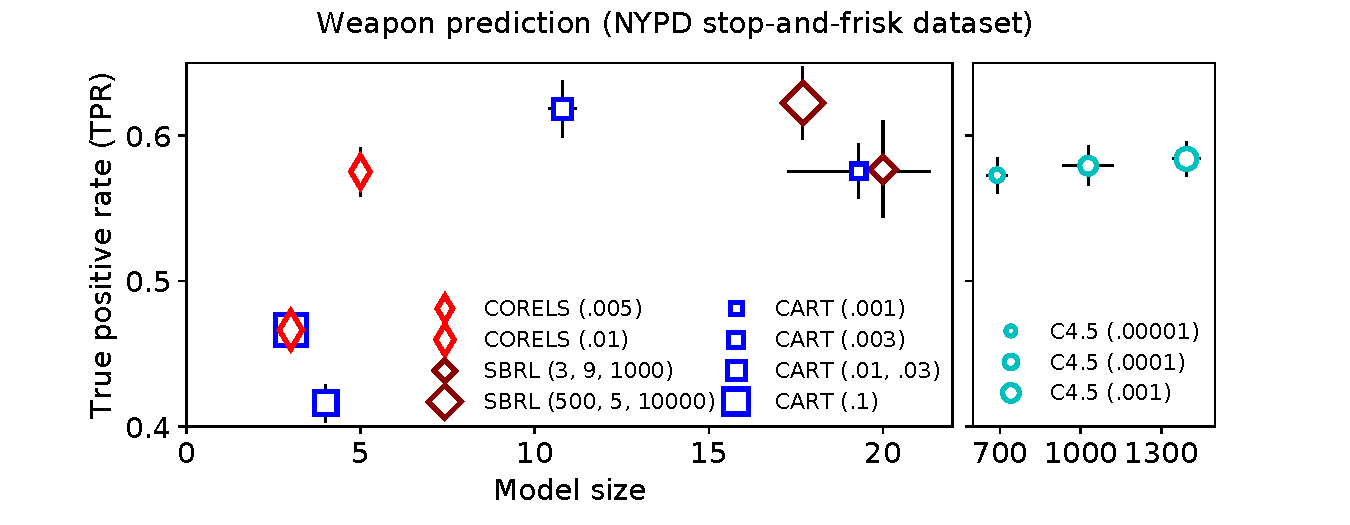
\includegraphics[trim={17mm, 0mm, 27mm, 0mm},
width=0.8\textwidth]{figs/cpw-noloc-sparsity-tpr.pdf}
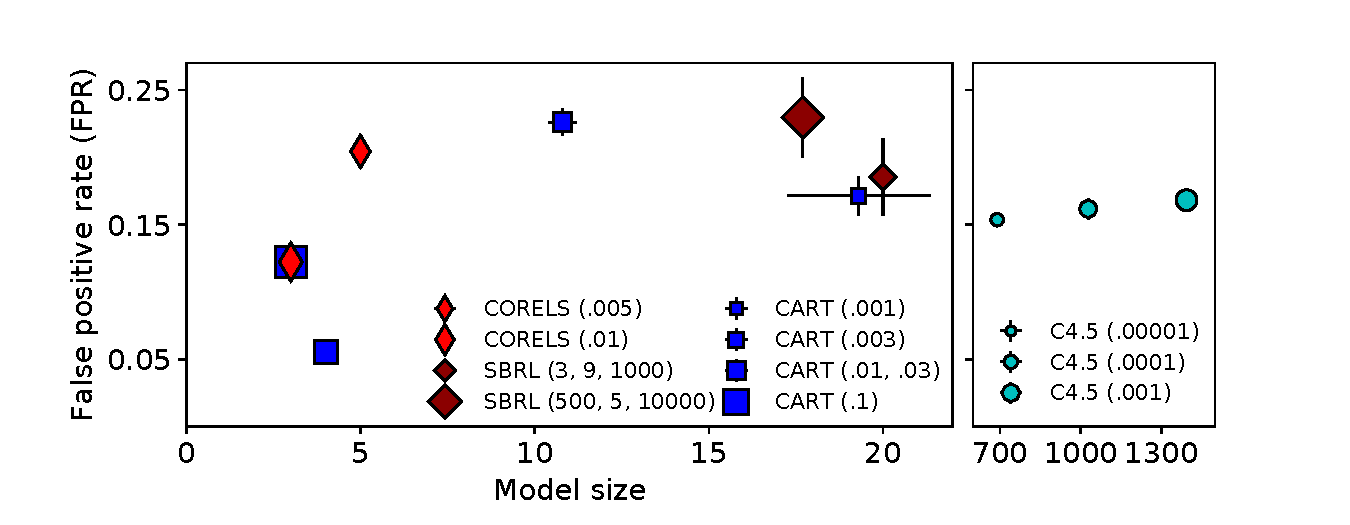
\includegraphics[trim={17mm, 10mm, 27mm, 4mm},
width=0.8\textwidth]{figs/cpw-noloc-sparsity-fpr.pdf}
\end{center}
\caption{TPR (top) and FPR (bottom)
for the test set, as a function of model size, across different methods,
for weapon prediction with the NYPD stop-and-frisk dataset (Feature Set~D).
%
In the legend, numbers in parentheses are algorithm parameters,
as in Figure~\ref{fig:sparsity-weapon}.
%
Legend markers and error bars indicate means and standard deviations,
respectively, across cross-validation folds.
%
%For CORELS and SBRL, we use ${M = 28}$ antecedents.
%
%CART with ${cp = 0.001}$ significantly overfits;
%C4.5 finds large models and dramatically overfits for all tested parameters.
C4.5 finds large models for all tested parameters.
}
\label{fig:sparsity-cpw}
\end{figure}
